%%%%%%%%%%%%%%%%%%%%%%%%%%%%%%%%%%%%%%%%%
% Arsclassica Article
% LaTeX Template
% Version 1.1 (10/6/14)
%
% This template has been downloaded from:
% http://www.LaTeXTemplates.com
%
% Original author:
% Lorenzo Pantieri (http://www.lorenzopantieri.net) with extensive modifications by:
% Vel (vel@latextemplates.com)
%
% License:
% CC BY-NC-SA 3.0 (http://creativecommons.org/licenses/by-nc-sa/3.0/)
%
%%%%%%%%%%%%%%%%%%%%%%%%%%%%%%%%%%%%%%%%%

%----------------------------------------------------------------------------------------
%	PACKAGES AND OTHER DOCUMENT CONFIGURATIONS
%----------------------------------------------------------------------------------------

\documentclass[
10pt, % Main document font size
a4paper, % Paper type, use 'letterpaper' for US Letter paper
oneside, % One page layout (no page indentation)
%twoside, % Two page layout (page indentation for binding and different headers)
headinclude,footinclude, % Extra spacing for the header and footer
BCOR5mm, % Binding correction
]{scrartcl}

%%%%%%%%%%%%%%%%%%%%%%%%%%%%%%%%%%%%%%%%%
% Arsclassica Article
% Structure Specification File
%
% This file has been downloaded from:
% http://www.LaTeXTemplates.com
%
% Original author:
% Lorenzo Pantieri (http://www.lorenzopantieri.net) with extensive modifications by:
% Vel (vel@latextemplates.com)
%
% License:
% CC BY-NC-SA 3.0 (http://creativecommons.org/licenses/by-nc-sa/3.0/)
%
%%%%%%%%%%%%%%%%%%%%%%%%%%%%%%%%%%%%%%%%%

%----------------------------------------------------------------------------------------
%	REQUIRED PACKAGES
%----------------------------------------------------------------------------------------

\usepackage[
nochapters, % Turn off chapters since this is an article        
beramono, % Use the Bera Mono font for monospaced text (\texttt)
eulermath,% Use the Euler font for mathematics
pdfspacing, % Makes use of pdftex’ letter spacing capabilities via the microtype package
dottedtoc % Dotted lines leading to the page numbers in the table of contents
]{classicthesis} % The layout is based on the Classic Thesis style

\usepackage{arsclassica} % Modifies the Classic Thesis package

\usepackage[T1]{fontenc} % Use 8-bit encoding that has 256 glyphs

\usepackage[utf8]{inputenc} % Required for including letters with accents

\usepackage{graphicx} % Required for including images
\graphicspath{{Figures/}} % Set the default folder for images

\usepackage{enumitem} % Required for manipulating the whitespace between and within lists

\usepackage{lipsum} % Used for inserting dummy 'Lorem ipsum' text into the template

\usepackage{subfig} % Required for creating figures with multiple parts (subfigures)

\usepackage{amsmath,amssymb,amsthm} % For including math equations, theorems, symbols, etc

\usepackage{varioref} % More descriptive referencing
\usepackage{color}
\usepackage{listings}
\usepackage{setspace}

\usepackage{lscape}


%----------------------------------------------------------------------------------------
%	THEOREM STYLES
%---------------------------------------------------------------------------------------

\theoremstyle{definition} % Define theorem styles here based on the definition style (used for definitions and examples)
\newtheorem{definition}{Definition}

\theoremstyle{plain} % Define theorem styles here based on the plain style (used for theorems, lemmas, propositions)
\newtheorem{theorem}{Theorem}

\theoremstyle{remark} % Define theorem styles here based on the remark style (used for remarks and notes)

%----------------------------------------------------------------------------------------
%	HYPERLINKS
%---------------------------------------------------------------------------------------

\hypersetup{
%draft, % Uncomment to remove all links (useful for printing in black and white)
colorlinks=true, breaklinks=true, bookmarks=true,bookmarksnumbered,
urlcolor=webbrown, linkcolor=RoyalBlue, citecolor=webgreen, % Link colors
pdftitle={}, % PDF title
pdfauthor={\textcopyright}, % PDF Author
pdfsubject={}, % PDF Subject
pdfkeywords={}, % PDF Keywords
pdfcreator={pdfLaTeX}, % PDF Creator
pdfproducer={LaTeX with hyperref and ClassicThesis} % PDF producer
}

\definecolor{Code}{rgb}{0,0,0}
\definecolor{Decorators}{rgb}{0.5,0.5,0.5}
\definecolor{Numbers}{rgb}{0.5,0,0}
\definecolor{MatchingBrackets}{rgb}{0.25,0.5,0.5}
\definecolor{Keywords}{rgb}{0,0,1}
\definecolor{self}{rgb}{0,0,0}
\definecolor{Strings}{rgb}{0,0.63,0}
\definecolor{Comments}{rgb}{0,0.63,1}
\definecolor{Backquotes}{rgb}{0,0,0}
\definecolor{Classname}{rgb}{0,0,0}
\definecolor{FunctionName}{rgb}{0,0,0}
\definecolor{Operators}{rgb}{0,0,0}
\definecolor{Background}{rgb}{0.98,0.98,0.98}

\lstnewenvironment{python}[1][]{
\lstset{
numbers=left,
numberstyle=\footnotesize,
numbersep=1em,
xleftmargin=1em,
framextopmargin=2em,
framexbottommargin=2em,
showspaces=false,
showtabs=false,
showstringspaces=false,
frame=l,
tabsize=4,
% Basic
basicstyle=\ttfamily\small\setstretch{1},
backgroundcolor=\color{Background},
language=Python,
% Comments
commentstyle=\color{Comments}\slshape,
% Strings
stringstyle=\color{Strings},
morecomment=[s][\color{Strings}]{"""}{"""},
morecomment=[s][\color{Strings}]{'''}{'''},
% keywords
morekeywords={import,from,class,def,for,while,if,is,in,elif,else,not,and,or,print,break,continue,return,True,False,None,access,as,,del,except,exec,finally,global,import,lambda,pass,print,raise,try,assert},
keywordstyle={\color{Keywords}\bfseries},
% additional keywords
morekeywords={[2]@invariant},
keywordstyle={[2]\color{Decorators}\slshape},
emph={self},
emphstyle={\color{self}\slshape},
%
}}{}

 % Include the structure.tex file which specified the document structure and layout

\hyphenation{Fortran hy-phen-ation} % Specify custom hyphenation points in words with dashes where you would like hyphenation to occur, or alternatively, don't put any dashes in a word to stop hyphenation altogether



%----------------------------------------------------------------------------------------
%	TITLE AND AUTHOR(S)
%----------------------------------------------------------------------------------------

\title{\normalfont\spacedallcaps{Detecting local events in the Twitter stream}} % The article title

\author{\spacedlowsmallcaps{Chris Pool}} % The article author(s) - author affiliations need to be specified in the AUTHOR AFFILIATIONS block

\date{} % An optional date to appear under the author(s)

%----------------------------------------------------------------------------------------

\begin{document}

%----------------------------------------------------------------------------------------
%	HEADERS
%----------------------------------------------------------------------------------------

\renewcommand{\sectionmark}[1]{\markright{\spacedlowsmallcaps{#1}}} % The header for all pages (oneside) or for even pages (twoside)
%\renewcommand{\subsectionmark}[1]{\markright{\thesubsection~#1}} % Uncomment when using the twoside option - this modifies the header on odd pages
\lehead{\mbox{\llap{\small\thepage\kern1em\color{halfgray} \vline}\color{halfgray}\hspace{0.5em}\rightmark\hfil}} % The header style

\pagestyle{scrheadings} % Enable the headers specified in this block


%----------------------------------------------------------------------------------------
%	Omslag
%----------------------------------------------------------------------------------------


\begin{titlepage}

\begin{figure}[h!] %  figure placement: here, top, bottom, or page

 
\includegraphics[width=4in]{Figures/ruglogo.eps} 
\end{figure}
\begin{center}

\vspace{30 mm}
\begingroup \linespread{1,75} \selectfont 
\textsc{\LARGE Detecting local events in the Twitter stream}\\[1,5cm]
\endgroup


by\\[0,5cm]
Chris Pool\\[2,5cm]


\end{center}
\vfill
\textbf{Bachelor thesis}\\
Information sciences\\
Chris Pool\\
S2816539\\
June 14, 2015



\end{titlepage}


%----------------------------------------------------------------------------------------
%	Title page
%----------------------------------------------------------------------------------------
\begin{titlepage}

\maketitle % Print the title/author/date block
\begin{figure}[htbp] %  figure placement: here, top, bottom, or page
   \centering
   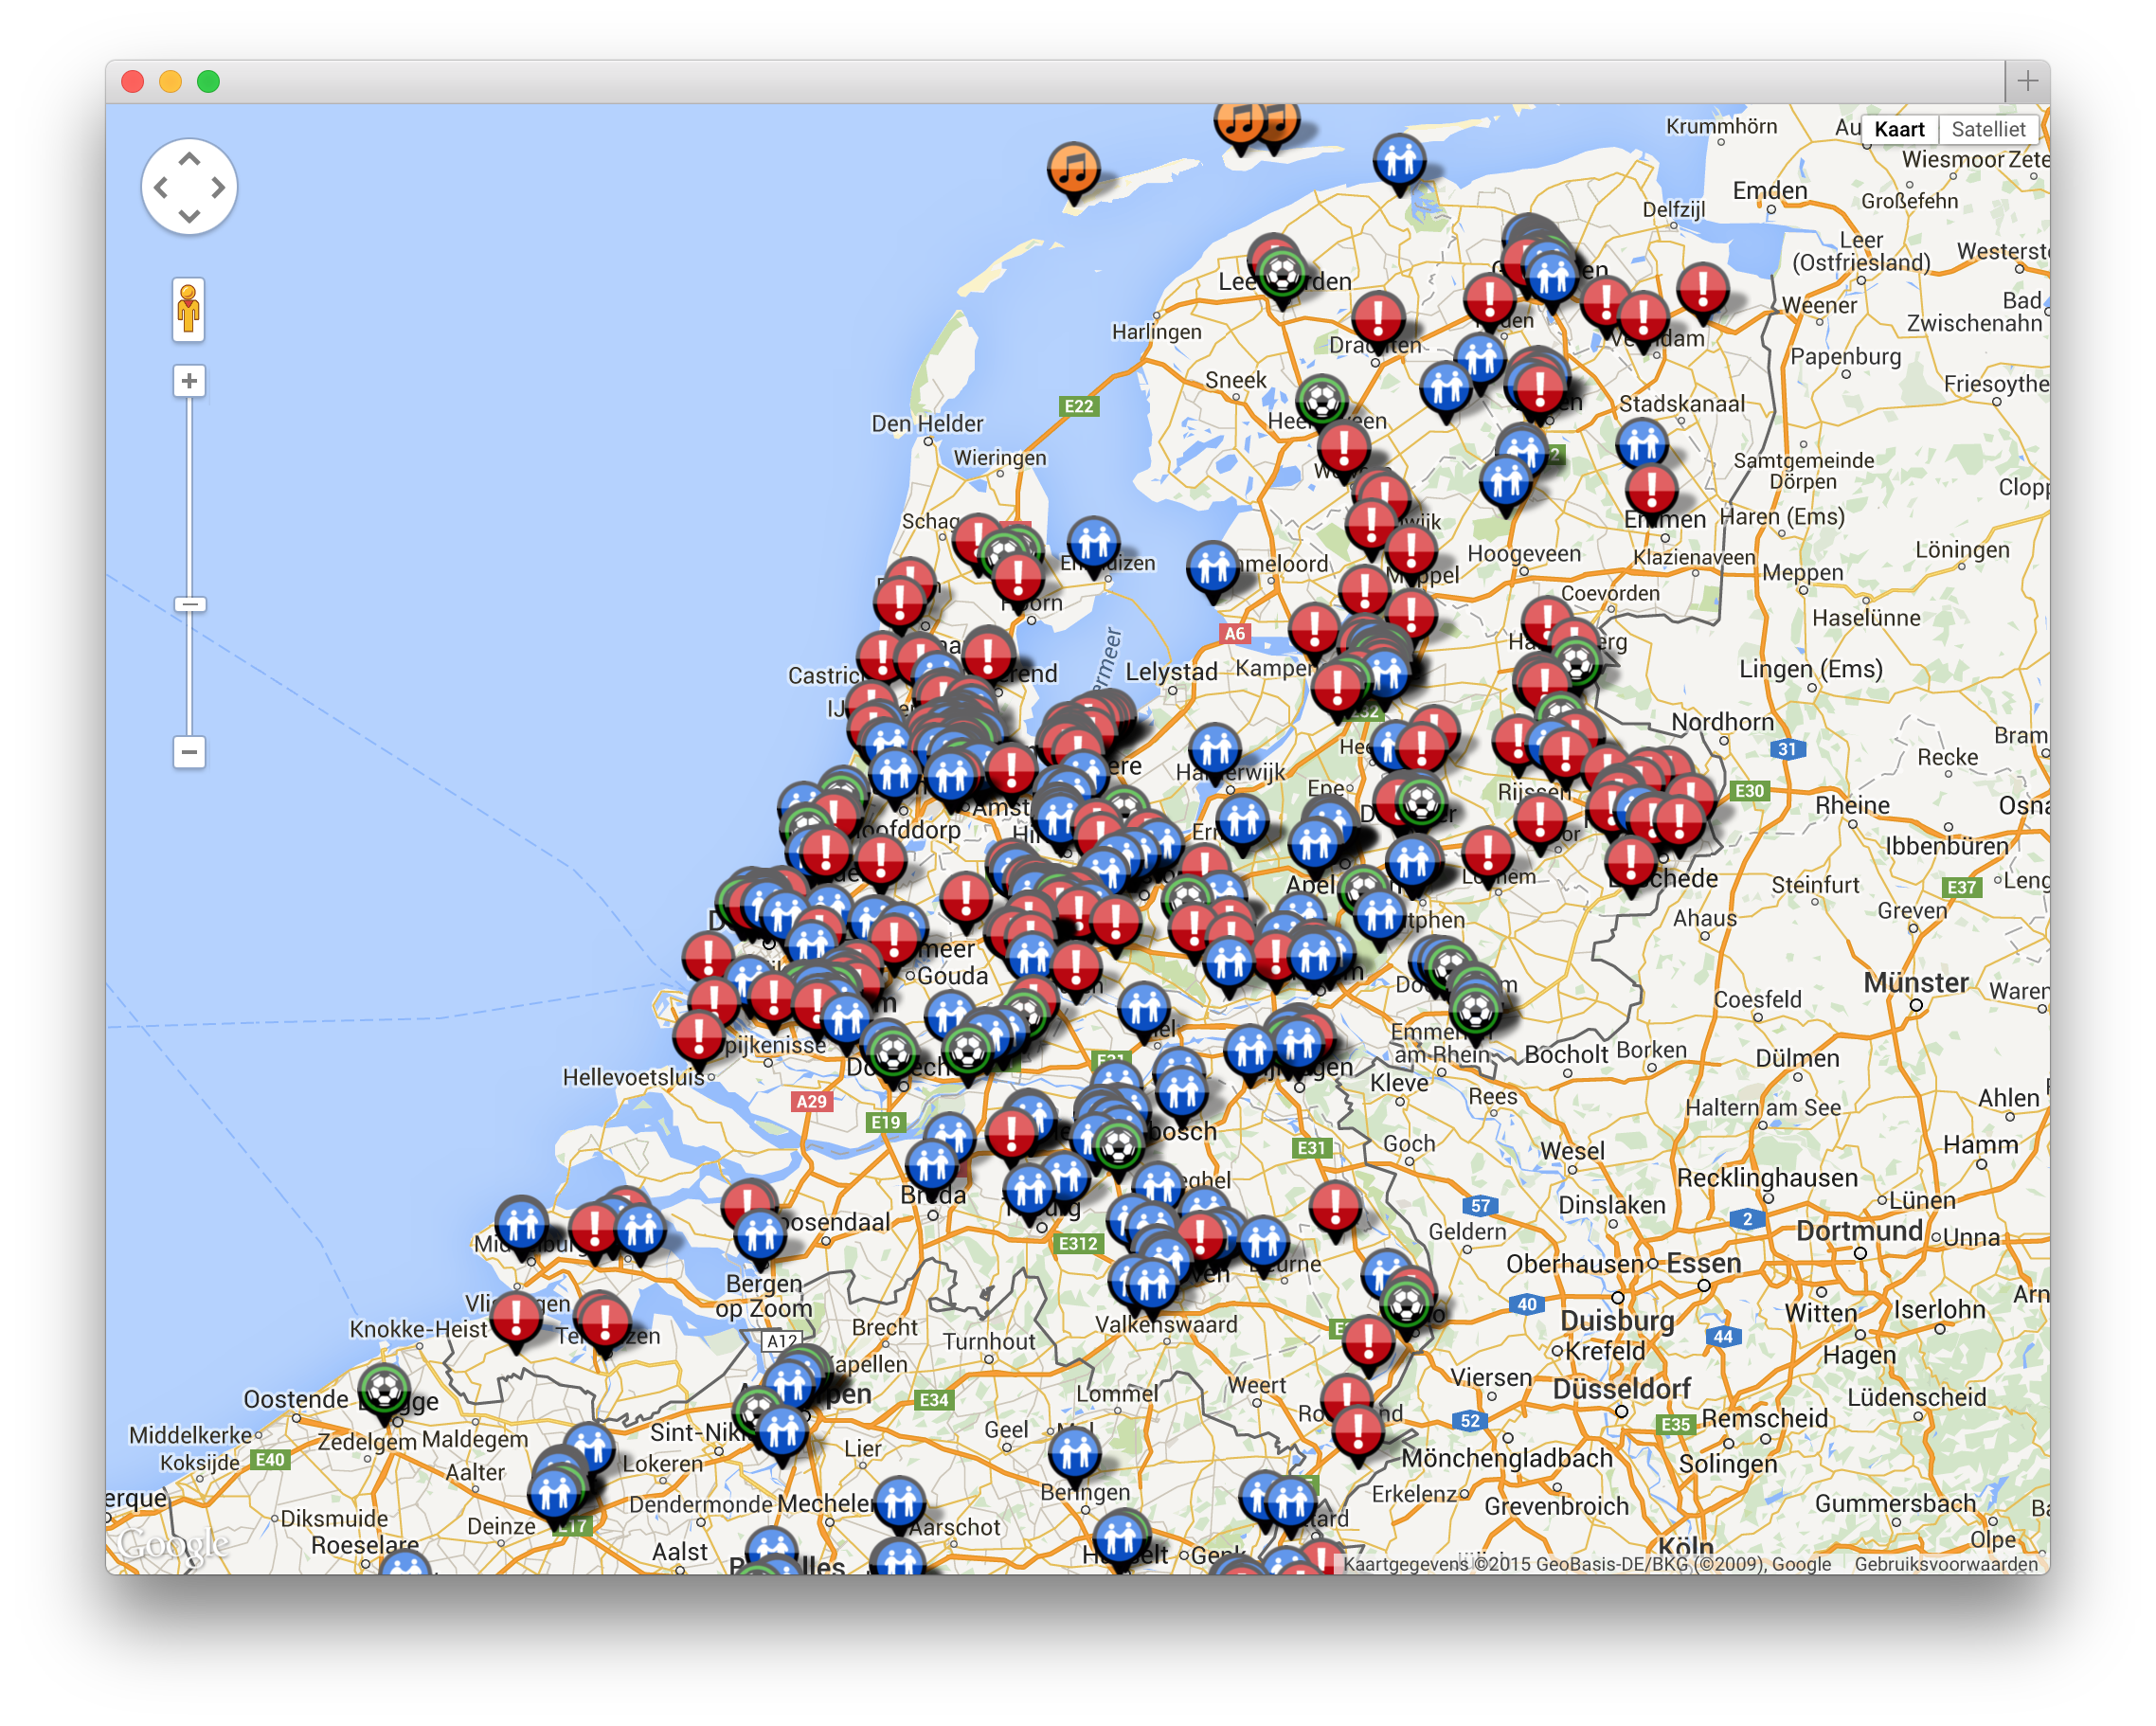
\includegraphics[width=4.5in]{voorkant.png} 
   \label{fig:gui}
\end{figure}
\thispagestyle{empty}
\end{titlepage}

%----------------------------------------------------------------------------------------
%	Preface
%----------------------------------------------------------------------------------------
\newpage
\section*{Preface} % This section will not appear in the table of contents due to the star (\section*)
This thesis is written as part of my Bachelor Information sciences at the University of Groningen that is part of my one year pre-master.  
\vl
I would like to thank my supervisors Malvina Nissim and Johan Bos for helping me during my research. I would also like to thank Rob van der Goot, PhD at the University of Groningen who helped me with creating a Named Entity Classifier.
\vl
Most of the programming is done together with David de Kleer, I would especially like to thank him for the pleasant collaboration.
\vl
\textit{Chris Pool}

%----------------------------------------------------------------------------------------
%	TABLE OF CONTENTS & LISTS OF FIGURES AND TABLES
%----------------------------------------------------------------------------------------
\newpage
\setcounter{tocdepth}{3} % Set the depth of the table of contents to show sections and subsections only
\tableofcontents % Print the table of contents

\listoffigures % Print the list of figures

\listoftables % Print the list of tables

\lstlistoflistings
%----------------------------------------------------------------------------------------
%	ABSTRACT
%----------------------------------------------------------------------------------------
\newpage
\section*{Abstract} % This section will not appear in the table of contents due to the star (\section*)
With the growing number of people using social media services like Twitter and the enormous amount of data available makes it interesting to use this data as a source of information about events that are taking place at a certain time and location. The goal of my research is to develop a system using tweets with geo-information that can detect events that take place at a specific location, for example concerts, football matches, fires and traffic jams and recognize the named entities in those events. Events that take place on a larger scale like elections and extreme weather conditions are ignored. 
\vl
The first step is collecting the data. I used the tweets available on the Karora server\footnote{Linux server available for students and staff of the University of Groningen}. This server stores all Dutch tweets and can be easily accessed. I downloaded all tweets with geo-information from May 2015 to use in developing the system. Tweets from the last two weeks in April 2015 are used to test the system.
\vl
The second step is to create clusters of these tweets, these clusters are potential \textit{event candidates}. We create these clusters by location and time. To make these \textit{event candidates} a algorithm is used called GeoHash, this  algorithm converts latitude and longitude coordinates into a hash, this hash indicates an area where the location is in. The more digits used for this hash, the smaller the area, and thus more accurate. For clustering by time I use the UNIX timestamp, this timestamp is a system that represents time in seconds since 1 January 1970.
\vl
The next step is to annotate the data, I and David de Kleer annotated the same datasets making it possible to calculate the inter-annotater agreement. With this annotated data we trained a Naive Bayes classifier. Using the development dataset as training data and the test dataset as test data this resulted in an accuracy of 84\%, with a upperbound of 86\& and baseline of 46\%\footnote{Baseline: Every event candidate is regarded as no event which is the largest category} we see this as a good result.
\vl
With the classified \textit{event candidates} using the categories: No event, Meeting, Entertainment, Incident, Sport and Other I try to detect named entities within those events. The Stanford Named Entity Recognizer was trained using automatically annotated tweets. The results are reasonable, but it shows the difficulty in detected entities in such short and noisy pieces of text.
\vl
The events, Including the named entities, are plotted on a Google map making it easy to check out the events.

%----------------------------------------------------------------------------------------

\newpage % Start the article content on the second page, remove this if you have a longer abstract that goes onto the second page

%----------------------------------------------------------------------------------------
%	INTRODUCTION
%----------------------------------------------------------------------------------------

\section{Introduction}

%waarom
With the growing number of people using social media services like Twitter and the enormous amount of data available makes it interesting to use this data as a source of information about events that are taking place at a certain time and location. About 3\% of all tweets contains geo-information\footnote{Based on my own data, see chapter 2 for literature research}. That looks like a small portion but because of the enormous amount of tweets available this gives great insights about the opinion of users at a certain location and can be very informative, for example to provide news items with more information about the opinion of people. 
\vl
This thesis describes a method of finding local events based on tweets with geo-information and categorizes them into 5 categories (No-event, Sport, Entertainment, Meeting and Incident). Also a method to find relevant information within those events about the location and people involved is described. Local events are events that take place in a certain radius (\begin{math}Z\end{math}) within a certain time interval (\begin{math}X\end{math}). For this research \begin{math}z= 0.5km , x= 2 hours\end{math}. 
\vl
My research question is: Is it possible to detect local events in the Twitter stream that take place in the Netherlands based on Tweets with geo-information, to see if you can detect what type of events take place and who the important people/organizations or topics are to make an interactive map of these events.
\vl
This thesis is devided in four chapters. The first chapter, related literature, describes the research that is done about this subject. The second chapter is the method section where I describe the methods I use for my experiment. In the third chapter i describe my experiment, all code I am referring to can also be found in my GitHub repository \footnote{http://www.github.com/chrispool/thesis}. In the final chapter you can find my conclusion.
%----------------------------------------------------------------------------------------
%	Related literature
%----------------------------------------------------------------------------------------
\newpage
\section{Related literature}

%twitter
Since the launch of Twitter in 2006 the popularity of this micro-blogging service is increasing rapidly (\citealt{statista}). With 302 million users sending about 500 million tweets per day this is a huge source of information. 
In the Netherlands the number of active users was 2.8 million in 2015 according to the research conducted by (\citealt{newcom}). The Netherlands still one of the countries with the highest twitter accounts to population ratio (\citealt{dawson}).
\vl
Using geo-information from tweets has been done in several researches, for example \citeauthor{sakaki2010earthquake} used geo-information of tweets to detect earthquakes by analyzing all tweets that contain certain keywords like \textit{earthquake} or \textit{shaking}. In literature this method of event detection is often referred to as spatio-temporal event detection. In the research by \cite{walther2013geo} they describe the process of detecting events in the Twitter stream, this research was the inspiration of my research and builds on several techniques they discuss. 
\vl
Current NER tools were designed to process large texts and perform poorly with tweets due to the noisy and short style of tweets, also the limit of 140 characters makes it difficult to recognize entities because the lack of context (\citealt{ner2011} and \citealt{liu2011ner}). A key feature for named entity recognition is the use of capital letters, unfortunately the use of capital letters in tweets if often less reliably and make it hard to recognize entities. According to \citeauthor{ner2011} the Stanford NER, a state of the art classifier, focusses to much on capital letters making it perform poorly with tweets.



%----------------------------------------------------------------------------------------
%	METHOD
%----------------------------------------------------------------------------------------
\newpage
\section{Method}
The goal of my research is to develop a system that can detect events that take place at a specific location, for example concerts, football matches, fires and traffic jams and recognize the named entities in those events. Events that take place on a larger scale like elections and extreme weather conditions are ignored. This chapter describes the methods used in my system and the motivation why I chose these methods.

\subsection{Clustering}
The first task is to cluster the tweets by location and time. There are several approaches in location clustering that can be used as discussed in the previous chapter. I wanted to use a clustering algorithm that potentially could work in real-time so it was necessary to look for an approach that was quick and accurate. GeoHash is is a system invented by Gustavo Niemeyer\footnote{http://en.wikipedia.org/wiki/Geohash} that converts latitude and longitude coordinates into a \textit{geoHash}. The hash represents an area where in the location is present. The length of the hash indicates the precision, more digits used indicates a smaller area, and thus a higher precision. If two locations share the same prefix it indicates (not always) that the locations are nearby. 
\begin{figure}[htbp] %  figure placement: here, top, bottom, or page
   \centering
   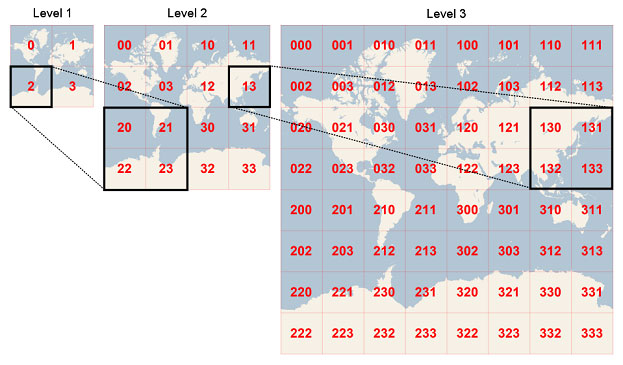
\includegraphics[width=4.5in]{geohash.jpg} 
   \caption{Geohash}
   \label{fig:geohash}
\end{figure}
\hfill \break Figure 1 illustrates how geoHash works. The first digit indicates which halve of the earth the area is on. The second digit divides that area in four areas and that continues resulting in table 1 that show the different lengths of the \textit{geoHash} and the accuracy of that length. Because the dimensions of the area are different at each latitude the values represent the worst-case scenario at the equator.

\begin{table}[h]
\caption[Geohash Precision]{Geohash Precision}
\begin{tabular}{|c|c|}
\hline
GeoHash length & Area width x height   \\ \hline
1              & 5,009.4km x 4,992.6km \\ \hline
2              & 1,252.3km x 624.1km   \\ \hline
3              & 156.5km x 156km       \\ \hline
4              & 39.1km x 19.5km       \\ \hline
5              & 4.9km x 4.9km         \\ \hline
6              & 1.2km x 609.4m        \\ \hline
7              & 152.9m x 152.4m       \\ \hline
8              & 38.2m x 19m           \\ \hline
9              & 4.8m x 4.8m           \\ \hline
10             & 1.2m x 59.5cm         \\ \hline
11             & 14.9cm x 14.9cm       \\ \hline
12             & 3.7cm x 1.9cm         \\ \hline
\end{tabular}
\end{table}
\newpage
There are several implementations of this algorithm in Python. I used the GeoHash library written in 2009 by Hiroaki Kawai\footnote{https://github.com/hkwi/python-geohash} because of the good documentation and excellent features. The function to calculate the \textit{geoHash} of a location requires the desired accuracy, latitude and longitude of that location and returns the \textit{geoHash} for that location as can be seen in code example 1. \vl

\begin{lstlisting}[language=Python, caption=Example of geoHash encoding]
lon = 52.348
lat = 6.2342
accuracy = 7

hash = geohash.encode(lon,lat,accuracy)
>>> print(hash)
u1k3y1c
\end{lstlisting}
The library also provides functions to calculate the neighboring geoHashes. This is useful because in a grid clustering approach border cases can occur.  This functionality can be used to merge those border cases as described in 4.3 Creating eventCandidates. \vl
For clustering timestamps the UNIX timestamp can be used. This is a system to represent time using the number of seconds since 1 January 1970. Python has build-in functions to deal with UNIX timestamps. The tweets are sorted on timestamp making it easy to make clusters of time series. The implementation of these functions can be found in chapter 3.3 Event Detection.

\newpage
\subsection{Classification}
After forming the potential events (\textit{eventCandidates}) the Event Candidates have to be classified as a specific event category or not an event.  NLTK provides excellent documentation and functions for classifying. \newline  NLTK enables you to use several classifiers:

\begin{itemize}[noitemsep]
\item ConditionalExponentialClassifier
\item DecisionTreeClassifier
\item MaxentClassifier
\item NaiveBayesClassifier
\item WekaClassifier
\item SVMClassifier (using scikit-learn)
\end{itemize}
In my experiment I have chosen to use the MaxEntClassifier, NaiveBayes and a SVM classifier. Using NLTK it was easy to train the classifiers. Each classifier requires the same format of train data making it easy to compare the results of the different classifiers.

\subsection{Named Entity Recognition}
For finding the important persons, organizations and locations I want to use Named Entity Recognition(NER). NER is the proces of labeling data with corresponding categories like person, organization or location. For example:

\begin {quote}
Na 14 minuten is het raak! 1-0 voor \textbf{Woudrichem(Organization)}. Doelpunt \textbf{Roy van Sonsbeek(Person)}
\end{quote}

As discussed in chapter 2 the standard NER classifiers perform poorly with tweets, therefore I decided to train my own classifier to detect named entities. With help from Rob van der Goot, PhD student at the University of Groningen I created an automatically annotated dataset. In the next chapter this process is explained in detail.
%----------------------------------------------------------------------------------------
%	Experiment and Evaluation
%----------------------------------------------------------------------------------------
\newpage
\section{Experiment and Evaluation}
For my experiment I worked together with David de Kleer in collecting the data and building the Python modules. The goal was to build a system that can detect events that take place at a specific location, for example concerts, football matches, fires and traffic jams and recognize the named entities in those events.  Events that take place on a larger scale like elections and extreme weather conditions are ignored. The input for this system are tweets that have coordinates that we cluster by location and time. These clusters of tweets are potential events (\textit{eventCandidates}) that the system classifies using the following categories: \newline

\begin{itemize}[noitemsep] % [noitemsep] removes whitespace between the items for a compact look
\item \textbf{Other (OTH)} All events that are other then the following categories 
\item \textbf{Meeting (MEE)} All events that are meetings or conferences 
\item \textbf{Entertainment (ENT)} All events that have to do with concerts, movies or theater
\item \textbf{No Event (NOE)} No Event
\item \textbf{Sport (SPO)} All events that have to do with sport 
\end{itemize}


\subsection{System architecture}
Python was used as the programming language for this system because of the excellent tools available to build a machine learning system. NLTK and Scikit learn are used for classifying \textit{eventCandidates}. GitHub\footnote{http://www.gitHub.com/chrispool/thesis} was used as file repository. The system consists of five different modules each containing multiple scripts. In this section the main properties of the modules are described. In the following sections the modules are explained in detail.

\begin{description}

\item[EventCandidates] 
The module that generates the \textit{eventCandidates} by clustering the tweets by \textit{geoHash} and timestamp and saves the result as a JSON file.  

\item[Annotater] 
The module that makes it possible for multiple judges to annotate the data created with the EventCandidates module and calculates the inter annotator agreement. 

\item[ClassifierCreator] 
The module that creates/trains the classifier(s) using the annotated \textit{eventCandidates.}

\item[EventDetective] 
The module that uses the trained classifier to classify eventCandidates and generate markers for the Google map.

\item[NER]
The module that uses the NER classifier that is explained in the Named Entity Recognition section of this chapter.  

\end{description}

\newpage
\subsection{Data collection}
For the experiment tweets are used that have geo-information. Using a simple Grep\footnote{Command-line utility for searching plain-text data sets for lines matching a regular expression } command it was possible to retrieve only tweets with this information from the Linux server \textit{Karora} \footnote{karora.let.rug.nl} that is available for students and staff of the University of Groningen. For our system we retrieved two datasets. One for training and developing our system that we call \textit{devset} and one for testing our final system that we call \textit{testset}
The \textit{devset} consists of Dutch tweets posted in March 2015 that we have downloaded from \textit{Karora}. In total there where 566.549 tweets with geo-information. That is about 3\% of the total number of tweets published in that month. The \textit{testset} consists of 165.848 tweets published in the second half of April 2015. The tweets are stored in a tab separated text file with the fields tweet, latitude, longitude, username and timestamp

\begin{quote}
@jokiecroky heb ze terug gebracht naar de plek waar ik ze heb opgehaald... volgende dag werd ik gebeld dat ze samen een mooi huisje hadden	5.106646 52.06455	TonyJuniorLive	2015-04-15 00:01:37 CEST Wed
\end{quote}


\subsection{Creating Event Candidates}
For clustering the tweets and preparing them for annotation and classification we use the EventCandidates module. This module processes all tweets from a given dataset and generates the \textit{eventCandidates} using four scripts. TweetPreprocessor.py, ClusterCreator.py, ClusterMerger.py and EventCandidates.py

\paragraph{TweetPreprocessor.py}reads the text file with tweets and tokenizes the tweets and removes the frequent occurring words from the tokens, convert the time string to a Unix timestamp and converts the latitude en longitude into a geoHash. The output of this script is a list of dictionaries where each dictionary is a tweet with the structure as found in code example 2.

\begin{lstlisting}[language=Python, caption=Tweet dictionary]
{'text': '@MrFrankLegs Daar gaan we. Een vicieuze cirkel ??', 
'lat': 52.964285, 
'geoHash': 'u1kjqcc', 
'localTime': '2015-04-24 10:54:16', 
'user': 'sandersierdsma', 
'tokens': ['@mrfranklegs', 'gaan', 'vicieuze', 'cirkel'], 
'lon': 5.923195, 
'unixTime': 1429865656}
\end{lstlisting}
\newpage
\paragraph{ClusterCreator.py} iterates over all tweet dictionaries and adds the tweet dictionary to a list in the new two-dimensional dictionary as seen in code example 3. With as first key the geoHash and the second key the Unix timestamp of the last added tweet. 
\begin{lstlisting}[language=Python, caption=Result dictionary]
clusters['u15y07t']['1429604082'] = [...list of tweet dictionaries...]
\end{lstlisting}
With this two-dimensional dictionary we can check for each tweet if we can add it to an existing \textit{eventCandidate} or that we have to create a new \textit{eventCandidate}. The code in code example 4 shows the clustering of the tweets.
\begin{lstlisting}[language=Python, caption=Cluster tweets]

#setting used for this experiment
self.MINUTES = 60

def __createClusters(self):
        for tweet in self.tweetDicts:
            geoHash = tweet["geoHash"]
            tweetTime = tweet["unixTime"]
            foundTime = tweetTime

            if geoHash in self.clusters:
                for times in self.clusters[geoHash].keys():
                    if times <= tweetTime <= times + self.MINUTES * 60:
                        foundTime = times
            
            self.clusters[geoHash][foundTime].append(tweet)
            if tweetTime != foundTime:
                # use new timestamp as key to keep event active
                self.clusters[geoHash][tweetTime] = self.clusters[geoHash][foundTime]
                # Remove old key
                del self.clusters[geoHash][foundTime] 
\end{lstlisting}

The output of this script is a dictionary with all clusters with the structure described in code example 3.
\newpage
\paragraph{ClusterMerger.py} checks if there are clusters that overlap in time and subject and are neighboring areas. For example the situation in figure 2, the tweets (red dots) are all about the same event and published in the same period but they are in two different areas.  

\begin{figure}[htbp] %  figure placement: here, top, bottom, or page
   \centering
   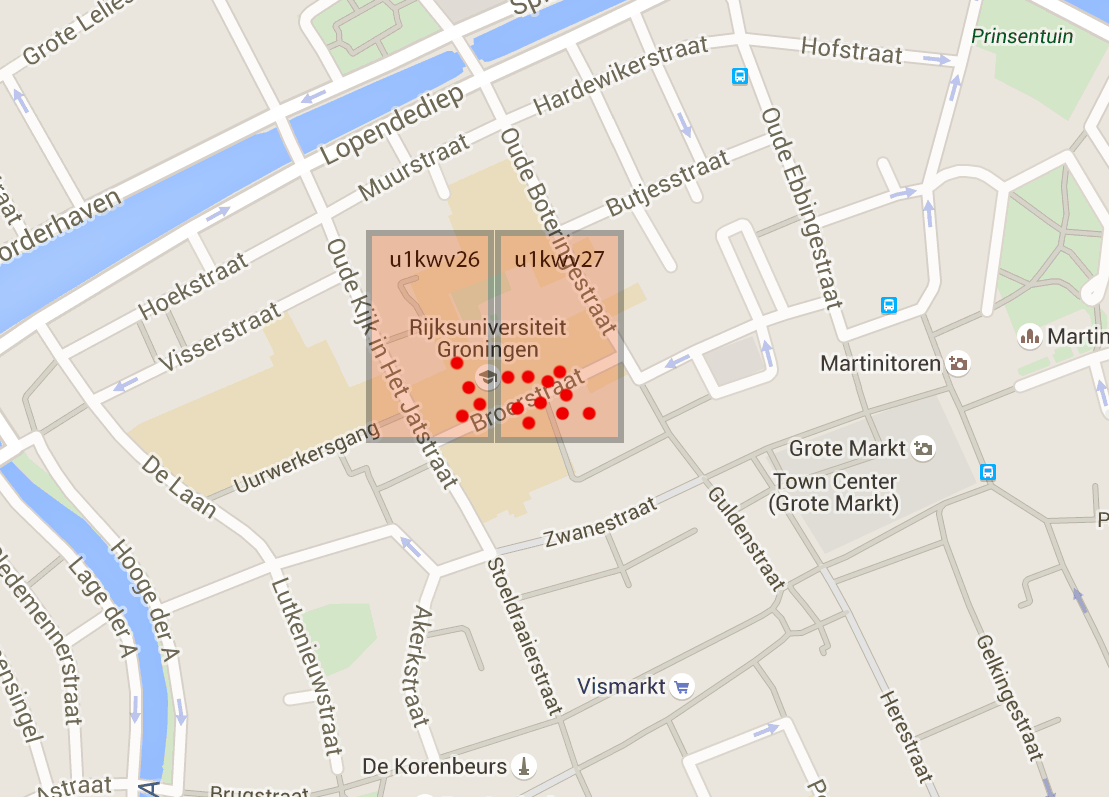
\includegraphics[width=3in]{bordercase.png} 
   \caption{Geohash border case}
   \label{Geohash border case}
\end{figure}
The ClusterMerger.py script tries to merge situations as described.  We do this by iterating over the \textit{eventCandidates} and calculate all neighbors of the current \textit{eventCandidate}. We then iterate over all neighboring areas, if an \textit{eventCandidate} is found we calculate the word overlap (code example 5) to see if the \textit{eventCandidates} is the same event. If that is the case we merge the cluster and continue the loop till all neighboring areas are checked.
\vl
We decided to iterate only once over all \textit{eventCandidates} because otherwise the area will be to big.
\vl
We calculate the word overlap to see if the two \textit{eventCandidates} have the same topic.  The function \textit{calculteWordOverlap}(code example 5) does that by looking at the 10 most common word in both clusters. For each word that overlaps a score of one point is awarded. If a hashtag or username overlaps two points are awarded. If a score exceeds the threshold the function returns true. 

\begin{lstlisting}[language=Python, caption=Calculate word overlap]
def _calculateWordOverlap(self,clusterA, clusterB):      
    wordsClusterA = self._getImportantWords(10, clusterA)
    wordsClusterB = self._getImportantWords(10, clusterB)
    result = {}
    
    #intersect the two lists and adding the scores
    for wordA, scoreA in wordsClusterA:
        for wordB, scoreB in wordsClusterB:
            if wordA == wordB:
                result[wordA] = scoreA + scoreB
                if wordA[0] == '#':
                    result[wordA] *= 2
                if wordA[0] == '@':
                    result[wordA] *= 2

    if sum(result.values()) > self.THRESHOLD:
        return True
    else:
        return False
\end{lstlisting}


\paragraph{EventCandidates.py} is the wrapper class for this module. This script generates all \textit{eventCandidates} using the scripts described above. This function requires two parameters. The first is the name of the text file with the unprocessed tweets. The second is the desired name of the dataset. This script saves a JSON file with all \textit{eventCandidates}.
\newpage
\subsection{Annotation}
This tool was used to annotate the two datasets: \textit{devset} and \textit{testset}. We annotated the \textit{devtest} in the beginning of our research, the \textit{testset} dataset in the final period of our research. The datasets where annotated with an interactive tool by two judges (figure 3). This tool also calculates the kappa score that can be used to determine the quality of annotation. The results of the annotation can be found in table 2. 

\begin{table}[h]
\caption[Annotation result]{Annotation result }
\begin{tabular}{|c|c|c|}
\hline
              & Kappa score & Accuracy \\ \hline
{\it devset}  & 0.79  & 87\%     \\ \hline
{\it testset} & 0.80  & 86\%     \\ \hline
\end{tabular}
\end{table}

The Kappa score indicates a good annotation. We regard the accuracy of 86\% as our upperbound.


\begin{figure}[htbp] %  figure placement: here, top, bottom, or page
   \centering
   \includegraphics[width=4in]{annotation.png} 
   \caption{Annotation tool}
   \label{fig:annotation}
\end{figure}


\begin{table}[h]
\caption[Confusion matrix testset annotation]{Confusion matrix development dataset annotation }
\begin{tabular}{lcccccc}
 & \multicolumn{1}{l}{\textbf{OTH}} & \multicolumn{1}{l}{\textbf{MEE}} & \multicolumn{1}{l}{\textbf{ENT}} & \multicolumn{1}{l}{\textbf{NOE}} & \multicolumn{1}{l}{\textbf{INC}} & \multicolumn{1}{l}{\textbf{SPO}} \\ \cline{2-7} 
\multicolumn{1}{l|}{\textbf{OTH}} & \multicolumn{1}{c|}{\textless1\textgreater} & \multicolumn{1}{c|}{.} & \multicolumn{1}{c|}{.} & \multicolumn{1}{c|}{2} & \multicolumn{1}{c|}{1} & \multicolumn{1}{c|}{1} \\ \cline{2-7} 
\multicolumn{1}{l|}{\textbf{MEE}} & \multicolumn{1}{c|}{21} & \multicolumn{1}{c|}{\textless207\textgreater} & \multicolumn{1}{c|}{7} & \multicolumn{1}{c|}{25} & \multicolumn{1}{c|}{.} & \multicolumn{1}{c|}{2} \\ \cline{2-7} 
\multicolumn{1}{l|}{\textbf{ENT}} & \multicolumn{1}{c|}{3} & \multicolumn{1}{c|}{.} & \multicolumn{1}{c|}{\textless20\textgreater} & \multicolumn{1}{c|}{5} & \multicolumn{1}{c|}{.} & \multicolumn{1}{c|}{.} \\ \cline{2-7} 
\multicolumn{1}{l|}{\textbf{NOE}} & \multicolumn{1}{c|}{14} & \multicolumn{1}{c|}{27} & \multicolumn{1}{c|}{18} & \multicolumn{1}{c|}{\textless619\textgreater} & \multicolumn{1}{c|}{9} & \multicolumn{1}{c|}{9} \\ \cline{2-7} 
\multicolumn{1}{l|}{\textbf{INC}} & \multicolumn{1}{c|}{1} & \multicolumn{1}{c|}{2} & \multicolumn{1}{c|}{.} & \multicolumn{1}{c|}{12} & \multicolumn{1}{c|}{\textless178\textgreater} & \multicolumn{1}{c|}{.} \\ \cline{2-7} 
\multicolumn{1}{l|}{\textbf{SPO}} & \multicolumn{1}{c|}{1} & \multicolumn{1}{c|}{.} & \multicolumn{1}{c|}{.} & \multicolumn{1}{c|}{5} & \multicolumn{1}{c|}{.} & \multicolumn{1}{c|}{\textless60\textgreater} \\ \cline{2-7} 
\end{tabular}

\end{table}
For the \textit{devset} we annotated 500 event candidates with these categories. In 86\% of the cases the judges agreed.
\begin{table}[h]
\caption[Confusion matrix devset annotation]{Confusion matrix test dataset annotation }
\begin{tabular}{lcccccc}
                                  & \multicolumn{1}{l}{\textbf{OTH}}            & \multicolumn{1}{l}{\textbf{MEE}}              & \multicolumn{1}{l}{\textbf{ENT}}            & \multicolumn{1}{l}{\textbf{NOE}}              & \multicolumn{1}{l}{\textbf{INC}}             & \multicolumn{1}{l}{\textbf{SPO}}    \\ \cline{2-7} 
\multicolumn{1}{l|}{\textbf{OTH}} & \multicolumn{1}{c|}{\textless.\textgreater} & \multicolumn{1}{c|}{.}                        & \multicolumn{1}{c|}{.}                      & \multicolumn{1}{c|}{.}                        & \multicolumn{1}{c|}{1}                       & \multicolumn{1}{c|}{.}              \\ \cline{2-7} 
\multicolumn{1}{l|}{\textbf{MEE}} & \multicolumn{1}{c|}{4}                      & \multicolumn{1}{c|}{\textless110\textgreater} & \multicolumn{1}{c|}{13}                     & \multicolumn{1}{c|}{9}                        & \multicolumn{1}{c|}{.}                       & \multicolumn{1}{c|}{3}              \\ \cline{2-7} 
\multicolumn{1}{l|}{\textbf{ENT}} & \multicolumn{1}{c|}{.}                      & \multicolumn{1}{c|}{.}                        & \multicolumn{1}{c|}{\textless8\textgreater} & \multicolumn{1}{c|}{2}                        & \multicolumn{1}{c|}{.}                       & \multicolumn{1}{c|}{.}              \\ \cline{2-7} 
\multicolumn{1}{l|}{\textbf{NOE}} & \multicolumn{1}{c|}{3}                      & \multicolumn{1}{c|}{19}                       & \multicolumn{1}{c|}{4}                      & \multicolumn{1}{c|}{\textless199\textgreater} & \multicolumn{1}{c|}{4}                       & \multicolumn{1}{c|}{2}              \\ \cline{2-7} 
\multicolumn{1}{l|}{\textbf{INC}} & \multicolumn{1}{c|}{1}                      & \multicolumn{1}{c|}{.}                        & \multicolumn{1}{c|}{.}                      & \multicolumn{1}{c|}{.}                        & \multicolumn{1}{c|}{\textless78\textgreater} & \multicolumn{1}{c|}{.}              \\ \cline{2-7} 
\multicolumn{1}{l|}{\textbf{SPO}} & \multicolumn{1}{c|}{.}                      & \multicolumn{1}{c|}{1}                        & \multicolumn{1}{c|}{2}                      & \multicolumn{1}{c|}{2}                        & \multicolumn{1}{c|}{.}                       & \multicolumn{1}{c|}{\textless60\textgreater} \\ \cline{2-7} 
\end{tabular}

\end{table}
\newpage
\subsection{Training classifiers}
With the annotation and the \textit{eventCandidates} ready we started with training the classifiers using the script ClassifierCreator.py. This module can be used in normal mode and in test mode. The first mode lets you select one dataset and the script divides the dataset in a 80/20 train / test set. The test mode lets you select two different datasets, one for training and the other for testing. The test mode was used for calculating the final statistics about our classifier.
\vl
Using the annotation and the \textit{eventCandidates} we start by preparing the training data. We have chosen to use two classifiers, one for classifying using words as features(\textit{categoryClassifier}). And a second classifier using metadata as features (\textit{eventClassifier}). The output of the \textit{categoryClassifer} is used as a feature in the eventClassifier.
\vl
We created featureSelector.py as a module that generates the features in the format required by NLTK. We designed this very modular so we could experiment with using different features and combinations of features. 
\vl
This function, as seen in code example 6, requires a list of the desired features and returns the features in a format suitable for training the classifier for a given cluster(\textit{eventCandidate}).\vl
The \textit{categoryClassifier} uses the N most frequent words as features. In order to calculate this feature the system needs to know all used words in the \textit{eventCandidates}, this is done while initializing the features module.

\begin{lstlisting}[language=Python, caption=Selecting features]
def getFeatures(self, candidate, features):
        returnFeatures = {}
        for feature in features:
            if feature in self.featureTypes:
                method = getattr(self, "_" + feature)
                if feature == 'wordFeatures':
                    wordFeatures = method(candidate)
                    #add word features to dictionary to be able to combine features
                    for key in wordFeatures:
                        returnFeatures[key] = wordFeatures[key]
                else:
                    returnFeatures[feature] = method(candidate)
            else:
                print("The feature", feature, "is not available.")

        return returnFeatures
\end{lstlisting}

With the features in the correct format we can train the classifiers. The code in code example 7 shows that adjusting the features is easy and allows us to experiment with different settings. The first for loop iterates over all test data and makes a tuple with two values from each \textit{eventCandidate} with at index 0 the features and at index 1 the label(category). It does the same for the train data. Training the classifier using NLTK can be done by using the train method that is available in the NLTK library. The classifierCreator module finally creates the statistics of the classifier that are used in the result section.

\begin{lstlisting}[language=Python, caption=Selecting features]
self.classifierBFeatures =  ['category', 'location','wordOverlapSimple','wordOverlapUser']
for candidate, label in self.testData:
            featuresB = self.featureSelector.getFeatures(candidate, self.classifierBFeatures)   
            self.featureKeys = featuresB.keys()
            self.testB.append((featuresB, label)) 
            
for candidate, label in self.trainData:
    featuresB = self.featureSelector.getFeatures(candidate, self.classifierBFeatures)
    self.featureKeys = featuresB.keys()
    self.trainB.append((featuresB, label))

self.classifierB = nltk.NaiveBayesClassifier.train(self.trainB)
\end{lstlisting}




\subsubsection{Feature selection}
The \textit{categoryClassifier} uses the most frequent words as features. The \textit{eventClassifier} uses the output of the first classifier as one of the features. This feature is by far the most valuable for the system. In table 4 the performance of the different features can be found. In appendix x the complete results can be found.


\begin{table}[h]
\caption[Effect of features]{Effect of features  }
\begin{tabular}{|l|l|}
\hline
                          & Accuracy \\ \hline
All features              & 0.84     \\ \hline
Category                  & 0.81     \\ \hline
Location                  & 0.51     \\ \hline
WordOverlapSimple         & 0.63     \\ \hline
WordOverlapUser           & 0.6      \\ \hline
WordOverlapUser, Category & 0.82     \\ \hline
\end{tabular}

\end{table}

\begin{description}

\item[Category]
The result of the classifier that uses the most frequent words as features. 

\item[Location]
The first 5 characters in the geoHash are used as a feature. It will be easier to detect events on locations were events often take place.

\item[wordOverlapSimple]
This feature is a numeric value that represents how many tweets consist of the same words. The score is calculated by counting the occurrences of each type and dividing it by the number of tweets. Hashtags get a bonus score.
\newpage
\begin{lstlisting}[language=Python, caption=Word overlap feature]
def _wordOverlapSimple(self, candidate):
        types = Counter()
        for tweet in candidate:
            types.update(set(tweet['tokens']))
        score = 0
        for t in types:
            if types[t] > 1:
                if t[0] == '#':
                    score += (types[t] * 2)
                else:
                    score += types[t]

        return round((score / len(candidate)) * 2) / 2
\end{lstlisting}

\item[WordOverlapUser]
This feature calculates the overlap of types among users. The score is the highest when all users use the same words. The result is the log of the score and rounded to 0.5.

\begin{lstlisting}[language=Python, caption=User word overlap feature]
def _wordOverlapUser(self, candidate):
        '''Calculate the overlap of features among users'''
        userTypes = defaultdict(list)
        types = Counter()

        for row in candidate:
            userTypes[row['user']].extend(row['tokens'])
        
        for user in userTypes:
            types.update(set(userTypes[user]))
        score = 0
        for t in types:
            if types[t] > 1: #ignore if only in one tweet
                if t[0] == '#':
                    score += (types[t] * 2)
                else:
                    score += types[t]

        if score > 1:
            s = log(float(score) * float(len(userTypes.keys()) )) 
            #return round((score * 2) / len(candidate))
            return round((s / len(candidate) )* 2 ) /2 
        else:
            return 0.0
\end{lstlisting}

\end{description}
\newpage
\subsubsection{Results event detection}
The event classifier performs good. It is a few procent less then the Upper bound  of 87\%. 

\begin{table}[h]
\caption[Results using all features]{Results using all features }
\begin{tabular}{l|l|l|l|l|l|l|l|l|l|}
\cline{2-10}
                          & \multicolumn{3}{c|}{Naive Bayes}                                         & \multicolumn{3}{c|}{Maximum Entropy}                                     & \multicolumn{3}{c|}{SVM}             \\ \cline{2-10} 
                          & \multicolumn{3}{c|}{Accuracy = 84\%}                                     & \multicolumn{3}{c|}{Accuracy = 83\%}                                     & \multicolumn{3}{c|}{Accuracy = 81\%} \\ \cline{2-10} 
                          & \multicolumn{1}{c|}{P} & \multicolumn{1}{c|}{R} & \multicolumn{1}{c|}{F} & \multicolumn{1}{c|}{P} & \multicolumn{1}{c|}{R} & \multicolumn{1}{c|}{F} & P          & R          & F          \\ \hline
\multicolumn{1}{|l|}{NOE} & 0.85                   & 0.90                   & 0.88                   & 0.83                   & 0.93                   & 0.88                   & 0.85       & 0.83       & 0.84       \\ \hline
\multicolumn{1}{|l|}{SPO} & 0.77                   & 0.49                   & 0.60                   & 0.77                   & 0.49                   & 0.60                   & 0.77       & 0.49       & 0.60       \\ \hline
\multicolumn{1}{|l|}{ENT} & 0.00                   & 0.00                   & 0.00                   & 0.00                   & 0.00                   & 0.00                   & 0.00       & 0.00       & 0.00       \\ \hline
\multicolumn{1}{|l|}{MEE} & 0.76                   & 0.79                   & 0.77                   & 0.79                   & 0.74                   & 0.76                   & 0.65       & 0.81       & 0.72       \\ \hline
\multicolumn{1}{|l|}{INC} & 0.97                   & 0.97                   & 0.97                   & 0.94                   & 0.94                   & 0.94                   & 1.00       & 0.97       & 0.99       \\ \hline
\multicolumn{1}{|l|}{OTH} & 0.00                   & 0.00                   & 0.00                   & 0.00                   & 0.00                   & 0.00                   & 0.00       & 0.00       & 0.00       \\ \hline
\end{tabular}

\end{table}


The different classifiers perform almost the same. This is mainly because the category feature is important for the results. If we don't use this feature the differences between the classifiers is bigger.

\begin{table}[h]
\caption[Confusion Matrix Naive Bayes]{Confusion Matrix Naive Bayes }
\begin{tabular}{|l|c|c|c|c|c|c|}
\hline
    & \multicolumn{1}{l|}{OTH} & \multicolumn{1}{l|}{MEE} & \multicolumn{1}{l|}{ENT} & \multicolumn{1}{l|}{NOE} & \multicolumn{1}{l|}{INC} & \multicolumn{1}{l|}{SPO} \\ \hline
OTH & \textless.\textgreater   & .                        & .                        & 1.                       & .                        & .                        \\ \hline
MEE & .                        & \textless82\textgreater  & 2                        & 14                       & .                        & 12                       \\ \hline
ENT & .                        & .                        & \textless.\textgreater   & 1                        & .                        & .                        \\ \hline
NOE & .                        & 27                       & 5                        & \textless179\textgreater & 1                        & 7                        \\ \hline
INC & .                        & .                        & .                        & 2                        & \textless76\textgreater  & .                        \\ \hline
SPO & .                        & 1                        & 1                        & 2                        & 1                        & \textless16\textgreater  \\ \hline
\end{tabular}


\end{table}

\begin{table}[h]
\caption[Confusion Matrix Maximum Entropy]{Confusion Matrix Maximum Entropy }
\begin{tabular}{|l|c|c|c|c|c|c|}
\hline
    & \multicolumn{1}{l|}{OTH} & \multicolumn{1}{l|}{MEE} & \multicolumn{1}{l|}{ENT} & \multicolumn{1}{l|}{NOE} & \multicolumn{1}{l|}{INC} & \multicolumn{1}{l|}{SPO} \\ \hline
OTH & \textless.\textgreater   & 1                        & .                        & .                        & .                        & .                        \\ \hline
MEE & .                        & \textless81\textgreater  & 2                        & 7                        & 2                        & 11                       \\ \hline
ENT & .                        & .                        & \textless.\textgreater   & .                        & 1                        & .                        \\ \hline
NOE & .                        & 26                       & 5                        & \textless186\textgreater & 1                        & 7                        \\ \hline
INC & .                        & 1                        & .                        & 4                        & \textless73\textgreater  & .                        \\ \hline
SPO & .                        & 1                        & 1                        & 2                        & 1                        & \textless16\textgreater  \\ \hline
\end{tabular}

\end{table}

\begin{table}[h]
\caption[Confusion Matrix SVM classifier]{Confusion Matrix SVM classifier }
\begin{tabular}{|l|c|c|c|c|c|c|}
\hline
    & \multicolumn{1}{l|}{OTH} & \multicolumn{1}{l|}{MEE} & \multicolumn{1}{l|}{ENT} & \multicolumn{1}{l|}{NOE} & \multicolumn{1}{l|}{INC} & \multicolumn{1}{l|}{SPO} \\ \hline
OTH & \textless.\textgreater   & 1                        & .                        & .                        & .                        & .                        \\ \hline
MEE & .                        & \textless89\textgreater  & 2                        & 31                       &                          & 14                       \\ \hline
ENT & .                        & .                        & \textless.\textgreater   & .                        &                          & .                        \\ \hline
NOE & .                        & 19                       & 5                        & \textless166\textgreater & 1                        & 4                        \\ \hline
INC & .                        & .                        & .                        & .                        & \textless73\textgreater  & .                        \\ \hline
SPO & .                        & 1                        & 1                        & 2                        & 1                        & \textless17\textgreater  \\ \hline
\end{tabular}

\end{table}
\newpage
\subsection{Event Detective}
This module uses the trained classifiers to generate an interactive map and adds the results of the Named Entity Recognition classifier described in the next section. It first asks you to select a classifier you want to use. The second step is to select a dataset you want to classify.
\vl
To create an interactive map we have chosen to use Google map because of the good documentation and excellent features. We generate a javascript file with all information about the markers we want to plot on the map. 
\begin{lstlisting}[language=Python, caption=Generate Javascript file]
def generateMarkers(self):
        print("Creating Google Maps markers & add WIKI links...")
        
        js = open('vis/map/js/markers.js','w')
        js.write('var locations = [')

        
        for tweets,label in self.events:
            writableCluster = ''
            gh = []
            i = 0
            avgLon = 0
            avgLat = 0
            #tweets = sorted(tweets, key=itemgetter('unixTime'));
                              
            for tweet in tweets:
                i = i + 1
                gh.append(tweet['geoHash'])
                avgLon += float(tweet["lon"])
                avgLat += float(tweet["lat"])
                # backslashes voor multiline strings in Javascript
                writableCluster += "{} {} {} {}<br/><br/>".format(tweet['localTime'], tweet['geoHash'], tweet['user'], tweet['text']).replace("'", "\\'")
            # Bepaal het Cartesiaans (normale) gemiddelde van de coordinaten, de afwijking (door vorm
            # van de aarde) zal waarschijnlijk niet groot zijn omdat het gaat om een klein vlak op aarde...
            # Oftewel, we doen even alsof de aarde plat is ;-)
            avgLon /= i
            avgLat /= i
            #writableCluster += "</br>" + str(ngrams).replace("'", "\\'")
            js.write("['{}', {}, {}, '{}'],".format(writableCluster,avgLat,avgLon,label))
        js.write('];')
        js.close()
\end{lstlisting}

\subsection{Named Entity Recognition}
The default NER tagger in NLTK is the Stanford NER classifier. This is according to many researches the best available. Unfortunately there are no classifiers trained using Dutch tweets and the performance of the available classifiers was so poor I decided to train my own classifier. Because of limited time I decided to automatically annotate the training data creating a silver standard.

\subsubsection{Data collection}
For creating the silver standard I used the approach described in xxx. by first selecting lists of Dutch words for each category I want to recognize (LOCATIONS, PERSONS, ORGANIZATIONS and MISC).  I used the word lists that also are used in the Alpino software\footnote{Alpino is a dependency parser for Dutch, developed in the context of the PIONIER Project Algorithms for Linguistic Processing. }
The wordlists are used to retrieve tweets that contain one or more of those words from the Karora machine. I downloaded 1 million tweets and wrote a Python script to create the training file that can be used to train your own classifier.

\subsubsection{Training}
The training file was used to train the classifier and by experimenting with the features. I also annotated about 100 tweets manually to calculate the precision and recall. The results can be found in table 12.


\subsubsection{Results}
There results are not great, compared to other researches .... the classifier misses a lot of entities. 

\begin{figure}[htbp] %  figure placement: here, top, bottom, or page
   \centering
   \includegraphics[width=4in]{ner.png} 
   \caption{NER example}
   \label{fig:example}
\end{figure}




\begin{table}[h]
\caption[NER Classifier trained with Tweets]{NER Classifier trained with Tweets }
\begin{tabular}{|l|l|l|l|l|l|l|}
\hline
Entity       & P      & R      & F1     & TP & FP & FN   \\ \hline
LOCATION     & 0,7333 & 0,7333 & 0,7333 & 11 & 4  & 4    \\ \hline
MISC         & 0,0909 & 0,500  & 0,1538 & 1  & 10 & 1    \\ \hline
ORGANIZATION & 0,7500 & 0,8824 & 0,8108 & 15 & 5  & 2    \\ \hline
PERSON       & 0,6154 & 0,5517 & 0,5818 & 16 & 10 & 13   \\ \hline
Totals       & 0,5972 & 0,6825 & 0,6370 & 43 & 29 & 20 \\ \hline
\end{tabular}

\end{table}


\clearpage
\newpage
\section{Conclusion and discussion}
\lipsum[10]
\lipsum[10]

\newpage
\section{Appendix}

\begin{landscape}
\begin{table}[h]
\begin{tabular}{|l|l|l|l|l|l|l|l|}
\hline
                          & accuracy & geen\_event    & sport          & entertainment  & bijeenkomst    & incident       & anders         \\ \hline
                          &          & P    R    F    & P    R    F    & P    R    F    & P    R    F    & P    R    F    & P    R    F    \\ \hline
All features              & 0.84     & 0.85 0.90 0.88 & 0.77 0.49 0.60 & 0.00 0.00 0.00 & 0.76 0.79 0.77 & 0.97 0.97 0.97 & 0.00 0.00 0.00 \\ \hline
Category                  & 0.81     & 0.85 0.82 0.84 & 0.73 0.46 0.56 & 0.00 0.00 0.00 & 0.66 0.84 0.74 & 0.99 0.97 0.98 & 0.00 0.00 0.00 \\ \hline
Location                  & 0.51     & 0.49 0.94 0.65 & 0.00 0.00 0.00 & 0.00 0.00 0.00 & 0.66 0.25 0.36 & 0.50 0.06 0.11 & 0.00 0.00 0.00 \\ \hline
WordOverlapSimple         & 0.63     & 0.60 0.85 0.71 & 0.00 0.00 0.00 & 0.00 0.00 0.00 & 0.57 0.33 0.42 & 0.77 0.83 0.80 & 0.00 0.00 0.00 \\ \hline
wordOverlapUser           & 0.6      & 0.57 0.93 0.71 & 0.00 0.00 0.00 & 0.00 0.00 0.00 & 0.00 0.00 0.00 & 0.66 0.90 0.76 & 0.00 0.00 0.00 \\ \hline
wordOverlapUser, category & 0.82     & 0.86 0.83 0.85 & 0.77 0.49 0.60 & 0.00 0.00 0.00 & 0.66 0.85 0.74 & 1.00 0.97 0.99 & 0.00 0.00 0.00 \\ \hline
\end{tabular}
\end{table}
\end{landscape}


%----------------------------------------------------------------------------------------
\bibliographystyle{authordate1}
\bibliography{chris}
\end{document}